\section{Introduction}
Cosmic Rays are protons and atomic nuclei with energies in the range
\SIrange{1e9}{1e21}{\electronvolt}, which move through space with nearly the
speed of light. Their spectrum (see \cref{fig:cr-whole-spectrum}) closely
resembles a power-law $j(E)\propto E^{-\alpha}$, on the basis of which one
can discuss some of their features:
\begin{itemize}
    \item At $E\sim\SI{1e15}{\electronvolt}$ (the \emph{knee}) the exponent
        steepens from $\alpha={2.5}\ldots{2.7}$ to $\alpha\approx3.1$;
        particles below this point can be detected directly, their flux is
        significantly anisotropic and their chemical composition is well
        understood.
    \item At $E\sim\SI{1e17}{\electronvolt}$ (the \emph{\nth{2} knee}) the
        exponent steepens again to $\alpha\approx3.3$.
    \item Particles with energies $\ge\SI{1e16}{\electronvolt}$ can not be
        observed directly, instead when colliding with molecules in the upper
        atmosphere a cascade of secondary particles is triggered
        (\emph{extensive air showers}; one primary cosmic rays produces
        $\ge\num{1e6}$ secondary particles). This makes it difficult to
        estimate their chemical composition, however current data strongly
        suggests that heavier nuclei are included. Their sources are as of
        today mostly uncertain.
    \item $E\sim\SI{1e18.5}{\electronvolt}$ is revered to as the \emph{ankle};
        there the exponent flattens to $\alpha\approx2.5$. With arrival rates
        of 1 particle km$^{-1}$ century$^{-1}$ at
        $E\sim\SI{1e19.5}{\electronvolt}$, the investigation of this range of
        the spectrum poses major challenges; the respective error bars in
        \cref{fig:cr-whole-spectrum-high} are of statistical nature.
    \item While for \inrange{E}{1e16}{1e19}{\electronvolt} the arrival
        directions are isotropic with a high confidence, recently
        significant anisotropies for $E\ge\SI{8e18}{\electronvolt}$ have been
        observed.
\end{itemize}

\begin{figure}[ht]
    \centering
    \begin{subfigure}[b]{.45\textwidth}
        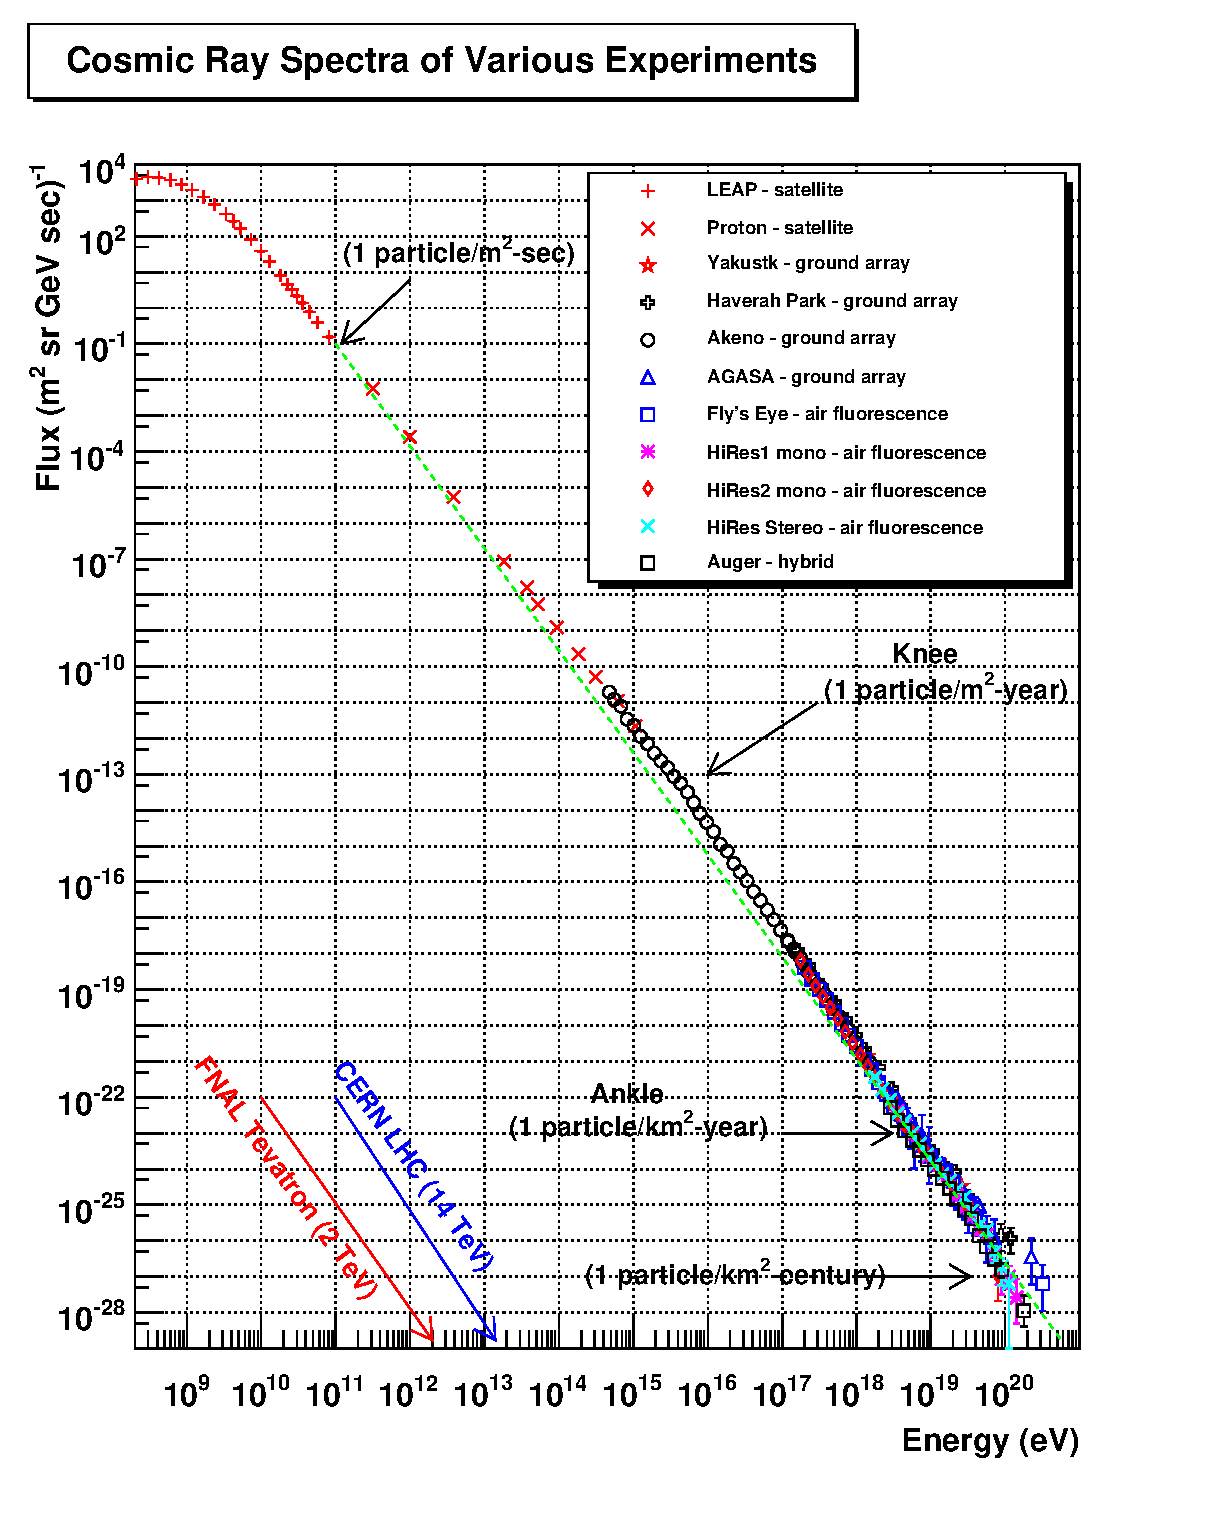
\includegraphics[width=\textwidth]{spectrum1}
        \caption{complete spectrum}
        \label{fig:cr-whole-spectrum-all}
    \end{subfigure}
    ~
    \begin{subfigure}[b]{.45\textwidth}
        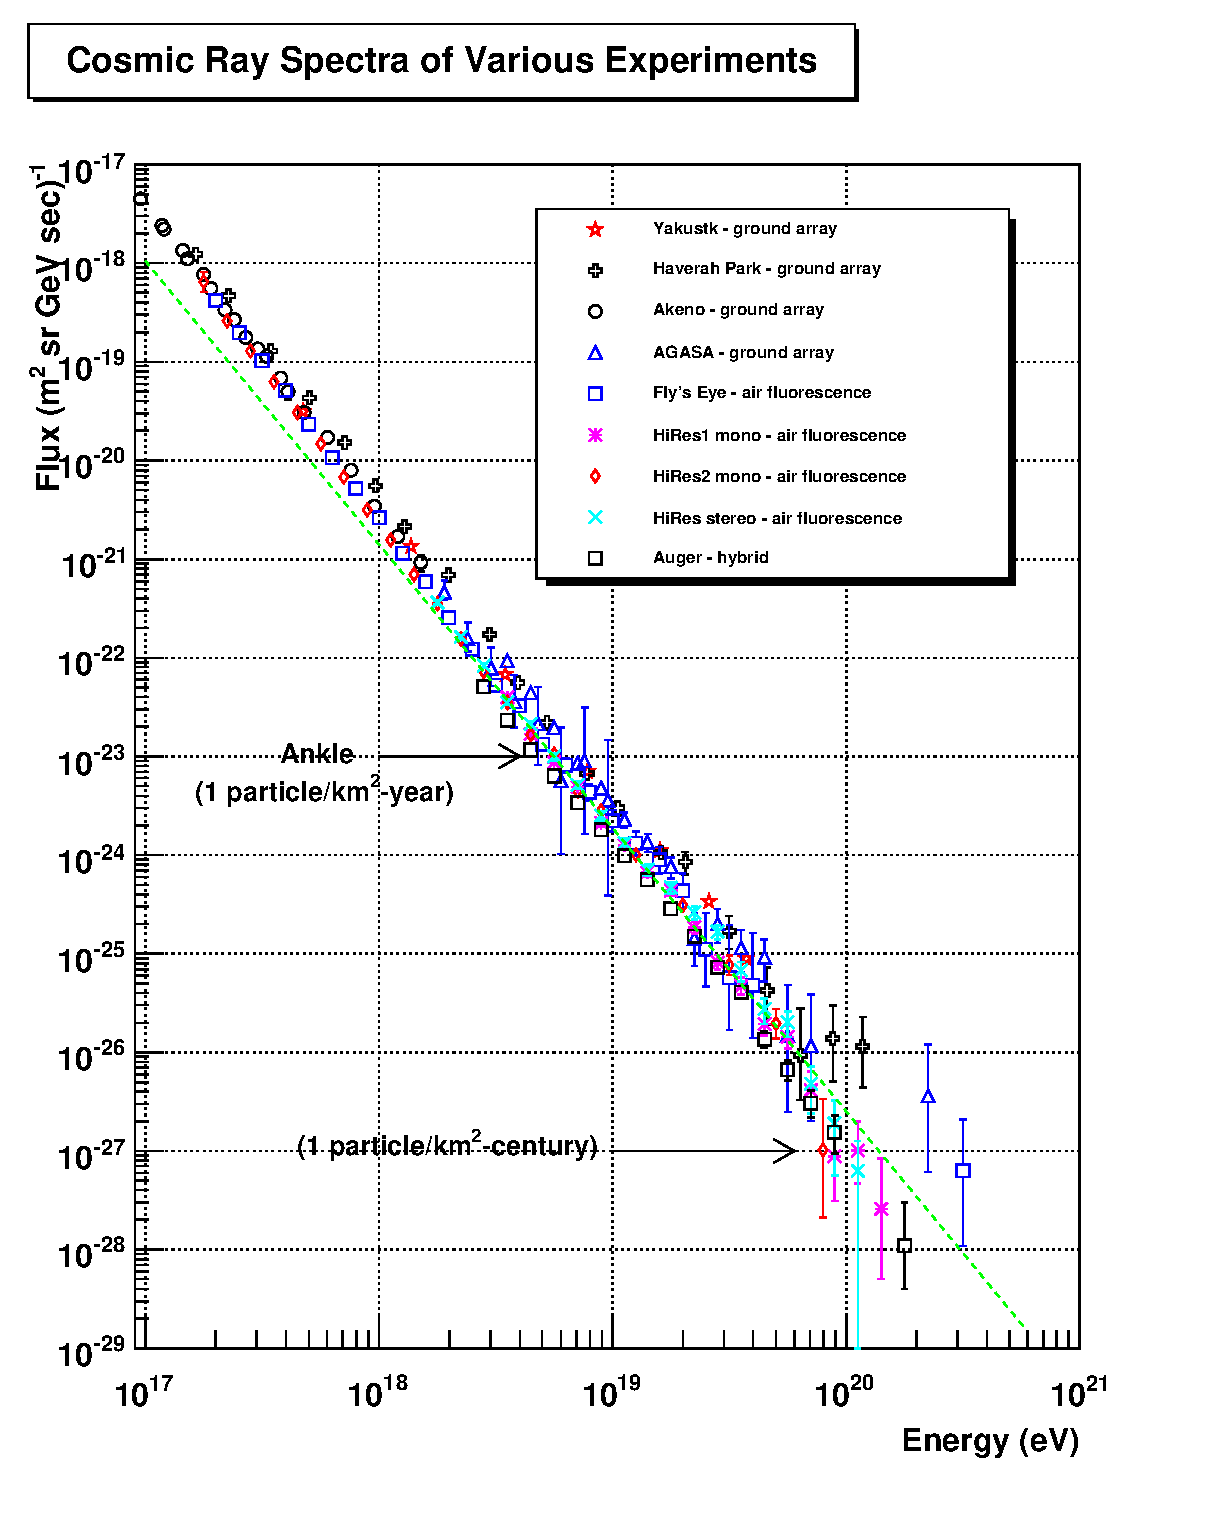
\includegraphics[width=\textwidth]{spectrum2}
        \caption{ultra-high energy regime}
        \label{fig:cr-whole-spectrum-high}
    \end{subfigure}
    \caption{Cosmic ray spectra of various experiments.
        Source\autocite{spectrum}}
    \label{fig:cr-whole-spectrum}
\end{figure}

This experiment is concerned with investigating the propagation of UHECR
(\emph{Ultra High Energy Cosmic Ray}) particles with energies above
\SI{1e18}{\electronvolt} using the Monte-Carlo code \CRPropa.


\section{Physical Fundamentals}
\subsection{Origin of UHECRs}
Which phenomenon is in principle able to accelerate particles to such large energies
(for reference: a particle with $E=\SI{3e20}{\electronvolt}$ has 23 million
times the LHC's collision energy of
$E_{\mathrm{LHC}}=\SI{13e12}{\electronvolt}$, but is still 40 million times
lower than the Planck energy $E_{\mathrm{P}}=\SI{1.2209e28}{\electronvolt}$)?

The isotropic distribution of arrival directions for particles with energies
$\ge\SI{1e16}{\electronvolt}$ suggests extra-galactic origins. This claim can
be supported by estimating the Lamor-radius of UHECRs in the interstellar
magnetic field:
\begin{equation}
    \Lamor=\frac{\gamma m v \sin\pitch}{ZeB}
    =\frac{pc}{Ze}\frac{\sin\pitch}{Bc}
    =\frac{R\sin\theta_{\mathrm{pitch}}}{Bc},
\end{equation}
where $R=pc/Ze$ is the particle's rigidity in volts, which is the same as the
particle's energy in electron-volts in the ultra-relativistic regime. With
a representative average galactic magnetic field strength of
$\SI{10}{\micro\gauss}$, one finds the values listed in \cref{tab:Lamor}.
Looking at these values, one finds that they are comparable to the estimated
half-thickness of the milky way's stellar disk of \SI{300}{\parsec} and its
radius of \SI{30}{\kilo\parsec}. One can argue, that as as soon as a particle's
Lamor-radius exceeds the half-thickness of it's source galaxy, it is able to
escape the galaxy's magnetic field.

\begin{table}[ht]
    \centering
    \sisetup{table-parse-only}
    \begin{tabular}{SSS}
        \toprule
        {$R/\si{\volt}$} & {$\Lamor/\si{\parsec}$ of a Proton} &
        {$\Lamor/\si{\parsec}$ of a \ce{^{56}Fe} nucleus} \\
        \midrule
        1e15 & .108 & 4.16e-3 \\
        1e17 & 10.8 & .416 \\
        1e19 & 1.08e3 & 41.6 \\
        1e21 & 108e3 & 4.16e3 \\
        \bottomrule
    \end{tabular}
    \caption{Lamor-radii for UHECR protons and iron nuclei with
        $B=\SI{10}{\micro\gauss}$}
    \label{tab:Lamor}
\end{table}

One class of possible extra-galactic particle accelerators are Active Galactic
Nuclei (AGN), which refer to galactic centers which outshine their host
galaxies and constitute the most luminous objects in the Universe. AGNs are
believed to be powered by mass-accreting super-massive black holes. Some of the
such arising accretion disks produce relativistic jets, \ie~highly collimated
beams of ionised particles accelerated close to the speed of light.
Additionally in such jet structures internal and external shocks might further
accelerate those particles. However the data available to date does not
sufficiently correlate the detected CRs with this kind of source.

Other possible sources include neutron stars, relativistic supernovae,
gamma-ray bursts or (going beyond the standard model) decay products of
super-massive topological defects in the underlying quantum field.


\subsection{Acceleration of Particles at Shocks}
Now, which processes are able to accelerate cosmic rays in such a way, that the
observed power spectrum is produced?
Promising candidates are astrophysical shocks, both locally (such as in solar
flares or relativistic jets) and on large scales (such as supernovae or
AGN), which was first described by Fermi (focusing on large-scale
phenomena)\autocite{Fermi1949}.

Considering some test particle in the vicinity of a shock, which is assumed to
experience an energy gain proportional to its energy during each encounter with
the shock $\Delta{E}=\zeta{E}$ and an initial energy $E_0$, one finds:
\begin{align*}
    E_1&=E_0+\Delta{E_0}=E_0(1+\zeta)\qc&\text{after the \nth{1} encounter} \\
    E_2&=E_1+\Delta{E_1}=E_0(1+\zeta)+\zeta{E_0}(1+\zeta)=E_0(1+\zeta)^2
    \qc&\text{after the \nth{2} encounter} \\
    &\vdots& \\
    E_n&=E_0(1+\zeta)^n\qc&\text{after the $n^{\text{th}}$ encounter}
    \numberthis\label{eq:En}
\end{align*}
It follows from \cref{eq:En}, that
\begin{equation}
    n={\log\left(\frac{E}{E_0}\right)}/{\log(1+\zeta)}
    \label{eq:num-enc}
\end{equation}
encounters are required to reach some energy $E$.

In a similar manner one can show, that the probability to remain in the
vicinity of the accelerating shock is $(1-\Pesc)^n$, where \Pesc~denotes the
escape probability per encounter.
Then the number of particles accelerated to energies greater than $E$ is
proportional to the sum of probabilities to remain, starting at the minimal
energy after $n$ encounters and taking into account all higher orders. This
eventually leads to a power law as shown in \cref{sec:app1}:
\begin{equation}
    N(>E)\propto\sum_{m=n}^{\infty}(1+\Pesc)^m
    \propto\frac{1}{\Pesc}\left(\frac{E}{E_0}\right)^{-\alpha},
    \label{eq:N-power}
\end{equation}
where the spectral index is approximately given by (for $\Pesc,\zeta\ll1$):
\begin{equation}
    \alpha\approx\frac{\Pesc}{\zeta}.
    \label{eq:alpha}
\end{equation}

Writing \cref{eq:N-power} as a differential energy spectrum yields:
\begin{equation}
    \boxed{%
        \dv{N(>E)}{E}\propto\left(\frac{E}{E_0}\right)^{-\alpha-1}
    }
    \label{eq:N-diff}
\end{equation}

Now, in order to determine the energy gain factor $\zeta$, two mechanisms of
acceleration are taken under closer consideration.


\subsubsection{\nth{2} order Fermi acceleration}
At first encounters of an ultra-relativistic ($E\approx pc$) test particle with
a moving cloud of plasma is discussed, where \emph{encounter} means entering
and exiting the cloud (see \cref{fig:fermi2}).

\begin{figure}[ht]
    \centering
    \includegraphics[width=.5\textwidth]{fermi2}
    \caption{Acceleration by a moving plasma cloud. Source\autocite{Gaisser}}
    \label{fig:fermi2}
\end{figure}

The particle with energy $E_1$ enters the cloud and diffuses by collisionless
scattering (without energy loss) on the irregularities in the magnetic field,
in such a way, that its \emph{average} motion coincides with that of the cloud.
In the following, primed quantities denote the rest-frame of the cloud, while
un-primed quantities denote the laboratory frame and the indices
\emph{1}/\emph{2} denote the state before/after the encounter.
Therewith the particle has in the rest-frame of the cloud the total energy
\begin{equation}
    E_1'=\gamma E_1(1-\beta\cos\theta_1)
    \label{eq:fermi2-e1p}
\end{equation}
with the Lorentz factor $\gamma$, the cloud's velocity $\beta=V/c$ and the
angle between the particle's and the cloud's velocity at entry $\theta_1$.
At the point of exiting, the particle's energy is unchanged in the cloud's
rest-frame ($E_1'=E_2'$), since only elastic scattering took place.
Transforming back into the laboratory frame then yields as the particle's
energy after the encounter
\begin{equation}
    E_2=\gamma E_2'(1+\beta\cos\theta_2')
    \label{eq:fermi2-e2}
\end{equation}
where $\theta_2'$ is the angle between the particle's and the cloud's velocity
at exit.

Now with the difference of \cref{eq:fermi2-e1p,eq:fermi2-e2} the energy change
can be computed:
\begin{align*}
    \frac{\Delta{E}}{E_1}
    &=\frac{\gamma{E_2'}(1+\beta\cos\theta_2')-\frac{E_1'}{\gamma(1-\beta\cos\theta_1)}}{\frac{E_1'}{\gamma(1-\beta\cos\theta_1)}}
    =\gamma(1-\beta\cos\theta_1)\gamma(1+\beta\cos\theta_2')-1\\
    &=\frac{1-\beta\cos\theta_1+\beta\cos_2'-\beta^2\cos\theta_1\cos\theta_2'}{1-\beta^2}-1.
    \numberthis\label{eq:dE}
\end{align*}

In order to find the average fractional energy gain per encounter,
$\cos\theta_1$ and $\cos\theta_2'$ need to be averaged:
\begin{align*}
    \langle\cos\theta_2'\rangle
    &=\frac{\int_{\text{all directions}}\dd{n}\cos\theta_2'}{\int_{\text{all
    directions}}\dd{n}}
    =\frac{\int_{-1}^{+1}\dd{\cos\theta_2'}\dv{n}{\cos\theta_2'}\cos\theta_2'}{\int_{-1}^{+1}\dd{\cos\theta_2'}\dv{n}{\cos\theta_2'}}
    =0,\numberthis
\end{align*}
since particles can leave the cloud isotropically, \ie~the probability for the
direction of exit is constant
\begin{equation}
    \dv{n}{\cos\theta_2'}=\mathrm{const.}\qc-1\le\cos\theta_2'\le1.
\end{equation}
Next, the probability for a collision of a cloud and a particle is proportional
to their relative velocity (with $v_{\mathrm{particle}}\approx c$)
\begin{equation}
    \dv{n}{\cos\theta_1}=\frac{c-V\cos\theta_1}{2c}\qc-1\le\cos\theta_1\le1,
\end{equation}
which gives
\begin{align*}
    \langle\cos\theta_1\rangle
    &=\frac{\int_{-1}^{+1}\dd{\cos\theta_1}\frac{c-V\cos\theta_1}{2c}\cos\theta_1}{\int_{-1}^{+1}\dd{\cos\theta_1}\frac{c-V\cos\theta_1}{2c}}
    =-\frac{V}{2c}\left[\frac{x^3}{3}\right]_{-1}^{+1}
    =-\frac{V}{3c}=-\frac{\beta}{3}.\numberthis
\end{align*}
Finally, one receives for the energy gain factor
\begin{equation}
    \zeta=\frac{\langle\Delta{E}\rangle}{E_1}
    =\frac{1+\frac{1}{3}\beta^2}{1-\beta}-1=\frac{\frac{4}{3}\beta^2}{1-\beta^2}
    \approx\frac{4}{3}\beta^2
    \label{eq:gain2}
\end{equation}
with the last approximation being valid for non-relativistic clouds,
\ie~$\beta\ll1$.

On average, particles gain energy according to \cref{eq:gain2}, however in
single encounters a particle might gain or lose energy depending on the entry
and exit angles.


\subsubsection{\nth{1} order Fermi acceleration}
The second situation deals with acceleration by a plane (infinitely spread out)
shock front moving with velocity $-\vec{u_1}$ (see \cref{fig:fermi1}).
The area in front of the shock is referred to as \emph{upstream} and the area
behind as \emph{downstream} region. The (shocked) downstream plasma moves away
from the shock front with velocity $\vec{u_2}$, where $u_2<u_1$, thus its
velocity in the lab frame is $\vec{V}=-\vec{u_1}+\vec{u_2}$.
Similar as above, \emph{encounter} means moving in and out of the shocked
region.

\begin{figure}[ht]
    \centering
    \includegraphics[width=.5\textwidth]{fermi1}
    \caption{Acceleration at a plane shock front. Source\autocite{Gaisser}}
    \label{fig:fermi1}
\end{figure}

\Cref{eq:dE} can still be applied here, with $\beta=V/c$ referring to the
downstream velocity. However when averaging the angular distributions, the
isotropy of entering and exiting directions only applies to the area behind or
in front of the shock respectively, \ie~the angles $\theta_2'$ and $\theta_1$
only take values in $[0,\pi/2]$ and $[-\pi/2,0]$ respectively and
the probabilities need to be projected onto the shock front and normalized
properly:
\begin{gather}
    \dv{n}{\cos\theta_2'}=2\cos\theta_2'\qc0\le\cos\theta_2'\le1 \\
    \dv{n}{\cos\theta_1}=2\cos\theta_1\qc-1\le\cos\theta_1\le0 \\
    \implies\langle\cos\theta_2'\rangle=-\langle\cos\theta_1\rangle=\frac{2}{3},
\end{gather}
which eventually yields for the energy gain factor
\begin{equation}
    \zeta=\frac{\langle\Delta{E}\rangle}{E_1}
    =\frac{1+\frac{4}{3}\beta+\frac{4}{9}\beta^2}{1-\beta^2}-1
    \approx\frac{4}{3}\beta=\frac{4}{3}\frac{u_1-u_2}{c},
    \label{eq:gain1}
\end{equation}
with the last approximation being valid for non-relativistic shocks,
\ie~$\beta\ll1$.

Due to the angular constraints, encounters with a plane shock front always
result in an energy gain.


\subsubsection{Acceleration at plane shock fronts}
The cosmic ray flux, which is to be accelerated by a shock front, first passes
from the upstream to the downstream region. This flux is found by projecting
some initially isotropic flux
$F_{\CR}^{\mathrm{iso}}=c\rho_{\CR}/4\pi$ onto the plane shock
front:
\begin{equation}
    F_{\CR}^{u\to{d}}
    =\int\limits_0^1\int\limits_0^{2\pi}\dd{\cos\theta}\dd{\phi}
    F_{\CR}^{\mathrm{iso}}\cos\theta
    =\int\limits_0^1\int\limits_0^{2\pi}\dd{\cos\theta}\dd{\phi}
    \frac{c\rho_{\CR}\cos\theta}{4\pi}
    =\frac{c\rho_{\CR}}{4}.
\end{equation}
The CR flux, which escapes from the shock front and is not being further
accelerated is given by the flux, which is on average transported away from the
shock front by the downstream plasma with speed $u_2$,
\ie~$F_\CR^{\mathrm{esc}}=\rho_{\CR}u_2$. The probability to
escape the region of acceleration is equal to the ratio of the fluxes, which
escape and which enter that region:
\begin{equation}
    \Pesc=\frac{F_{\CR}^{\mathrm{esc}}}{F_{\CR}^{u\to{d}}}
    =\frac{\rho_\CR u_2}{c\rho_\CR/4}=\frac{4u_2}{c}
    \label{eq:Pesc}
\end{equation}

Having estimated the energy gain factor \cref{eq:gain1} and the escape
probability \cref{eq:Pesc}, the spectral index \cref{eq:alpha} can finally be
obtained:
\begin{equation}
    \alpha=\frac{\Pesc}{\zeta}=\frac{4u_2/c}{4(u_1-u_2)/3c}=\frac{3}{u_1/u_2-1},
    \label{eq:alpha-plane-shock}
\end{equation}
where the ratio $u_1/u_2$ denotes the \emph{compression ratio} $r$ of the
shock. For a perpendicular MHD shock in the limit of large upstream flow
energy, one has (as shown in \cref{sec:app2}):
\begin{equation}
    r=\frac{\gamma+1}{\gamma-1}.
\end{equation}
Assuming mono-atomic gas with adiabatic index $\gamma=5/3$ gives $r=4$, \ie~for
the aforementioned assumptions the maximum jump of the plasma quantities at the
discontinuity of the shock is by a factor of four.

Therewith the spectral index becomes $\alpha=1$ and yields for the
differential energy spectrum \cref{eq:N-diff}:
\begin{equation}
    \boxed{\dd{N}\propto E^{-2}\dd{E}}
    \label{eq:N-power-2}
\end{equation}


\subsection{GZK Cutoff}
The here investigated UHECR protons have such large Lorentz factors, that the
photons of the Cosmic Microwave Background (CMB) get blue-shifted into the
$\gamma$-regime in the proton's rest frame.
With the proton being bombarded by high-energy $\gamma$-photons, pions are
created:
\begin{align*}
    \ce{p + $\gamma$ &-> n + $\pi^+$ -> n + $\nu^+ + \nu_{\mu}$} \\
    \ce{p + $\gamma$ &-> p + $\pi^0$ -> p + $\gamma + \gamma$}
\end{align*}
Integrating over the black-body spectrum of the CMB and over all angles, one
finds the threshold for \textbf{Photo-Pion Production} to be
$E\approx\SI{5e19}{\electronvolt}$. Further the mean free path for a single
scattering with a CMB photon can be estimated to
$\lambda\approx\SI{1e23}{\metre}\approx\SI{3}{\mega\parsec}$. The energy of the
so created pion is $\gamma m_{\pi} c^2$ and thus the fractional energy loss of
the proton is $\Delta{E}/E\approx m_{\pi}/m_p\approx 1/10$. Therefore, the
total mean free path for the proton to loose all its energy is about
\SI{30}{\mega\parsec}, which means there must be a cutoff in the energy
spectrum at \SI{5e19}{\electronvolt} if the cosmic rays originate from further
away (as first discussed by Greisen, Kuz'min and Zatsepin). However no such
cutoff is apparent in the measured spectrum, which means that either the cosmic
rays sources are located closer than \SI{30}{\mega\parsec} or the cosmic rays
are constituted of heavier nuclei such as iron instead of protons, which would imply
a smaller Lorentz factor for the same particle energy and thus the cutoff being
located at even higher energies.

Another process is $e^-$-$e^+$ \textbf{Photo-Pair Production}, where a
$\gamma$-photon with at least twice the rest energy of an electron is converted
into an electron and a positron. This only happens in the vicinity of a
heavier particle (such as a proton or heavier nucleus) in order to account for
conservation of momentum. A similar calculation as above can be carried out for
this process to yield a threshold for the proton energy of about
\SI{1e18}{\electronvolt}. While the cross-section here is 40 times larger
compared to photo-pion production, the fractional energy loss of the proton is
only $\Delta{E}/E\approx10^{-3}$, causing a 25 times longer
loss-scale.

In the case of the UHECRs being nuclei, \textbf{Photo-Disintegration} needs
also to
be considered: when the $\gamma$-photons in the rest frame of the nucleus reach
energies comparably to the binding energy per nucleon (which is of order
\SI{10}{\mega\electronvolt}), the absorption of such a photon leads to the
excitation of one or two nucleons and their subsequent ejection from the
nucleus. The smaller nucleus afterwards continues its disintegration via
further photo-disintegration and radioactive decay. From the Lorentz factor
necessary for this process, one finds for the threshold energy
$E\ge{A\times10^{18}}\si{\electronvolt}$, leading to a expected cutoff at about
\SIrange{1e19}{1e20}{\electronvolt}. The associated loss-scale is expected to
be smaller than with photo-pion production.

All of the above processes can also occur in interaction with Cosmic Infrared
Background (IRB), which is mostly due to galaxy formation and starlight absorbed
and re-emitted by interstellar dust. The hereafter performed simulations
use the model by Gilmore\autocite{Gilmore2012}.


\subsection{Turbulent Magnetic Fields}
\label{sec:intro-turbulence}
At first -- from a naive perspective -- the observed isotropy is unexpected, as
one would expect particles with such high energies to not be significantly
affected by magnetic fields and point directly back to their sources. That this
is not the case, can be explained by resonant scattering of those particles
with turbulent magnetic fields.

How generation and maintenance of large-scale magnetic fields in the Universe
theoretically work, is still unsolved as of today. Additionally -- while the
large-scale structure of galactic magnetic fields can be understood by
measuring the polarization of synchrotron radiation and taking Faraday rotation
into account -- putting observational constrains on the field strength
of extra-galactic magnetic fields is rather difficult.

For simplicity in this experiment a uniform isotropic turbulent field is
assumed, which is characterized by the root mean squared strength
$\Brms=\sqrt{\langle{B^2(x)}\rangle}$ and the distribution of magnetic energy
$w$, which -- according to Kolmogorov theory -- follows a power-law in Fourier
space between the maximum and minimum wave-numbers \kmin~and \kmax, which
describes how much energy is contained in eddies with wave-number $k$:
\begin{equation}
    w(k)=\frac{\Brms^2}{8\pi}k^{-m}\frac{(m-1)\kmin^{m-1}}{1-(\kmax/\kmin)^{m-1}},
\end{equation}
where a Kolmogorov spectrum with spectral index $m=5/3$ is chosen.
In a turbulent system energy is injected at the maximum length scale
$\lmax=2\pi/\kmin$ and from there is transferred through wave interactions to
the minimum length scale $\lmin=2\pi/\kmax$, where it dissipates.
Additionally, one can compute the correlation length $l_c$, which is the
characteristic length scale on which the magnetic field varies, and can be
thought of as roughly the size of the largest eddy in the system. For uniform
isotropic turbulent flow, Kolmogorov turbulence and $\lmin\ll\lmax$ one has:
\begin{equation}
    l_c=\frac{8\pi^2}{\Brms^2}\int\limits_{0}^{\infty}\frac{\dd{k}}{k}w(k)
    =\frac{\lmax}{2}\frac{m-1}{m}\frac{1-(\lmin/\lmax)^m}{1-(\lmin/\lmax)^{m-1}}
    \approx\frac{\lmax}{5}.
\end{equation}

A useful quantity to classify the relation of the particle with the magnetic
field is the dimensionless rigidity $r=\Lamor/l_c$ (not to be confused with the
rigidity in volts $R=pc/Ze$ discussed above), where $\Lamor=E/Ze\Brms c$ is the
particle's Lamor-radius in the ultra-relativistic limit (\ie~$E\approx pc$).

Now, the particle undergoes resonant scattering if $k\cos\pitch=1/\Lamor$:
\begin{itemize}
    \item upper limit:
        \[\kmin\le\frac{1}{\Lamor} \implies \rho\le\frac{5}{2\pi}\approx1\]
        $\rho\approx1$ divides the resonant from the quasi-ballistic regime; for
        $\rho\gg1$ the particle propagates quasi-rectilinear.
    \item lower limit:
        \[\kmax\ge\frac{1}{\Lamor} \implies
            \rho\ge\frac{5}{2\pi}\frac{\lmin}{\lmax}\approx\frac{\lmin}{\lmax}\]
        At $\rho\ll1$ particle propagation is also affected by magnetic field
        line random walks.
\end{itemize}
Therefore, the resonant scattering regime at which particle propagation is
diffusive is given by:
\begin{equation}
    \frac{\lmin}{\lmax}<\rho<1
    \label{eq:resontant-scattering}
\end{equation}


\subsection{Propagation of UHECRs}
\subsubsection{CRPropa3}
The propagation of cosmic rays can be obtained by solving either the
Fokker-Planck equation for a distribution of many particles
or the equation of motion according to the Lorentz force for a single particle.
Since for both cases no analytical solutions exist (due to the complicated
setting of the problem), one approaches this problem
numerically. With \CRPropa~a tool is provided for this task, which can compute
the propagation of cosmic rays -- including deflection by turbulent magnetic
fields, several energy loss processes through interaction with background
photon fields and nuclear decay -- over several orders of magnitude in energy
and length scales (hundreds of megaparsecs to kiloparsec).

Here the simplest case of solving the equation of motion of single particles is
considered, whose initial conditions are randomly drawn from a source probability
distribution. In order to obtain reliable results (\ie~with negligible
statistical fluctuations) this needs to be repeated for a large number of
particles.


\subsubsection{The Monte-Carlo method}
The basic idea behind the Monte-Carlo approach is to repeatedly perform an
experiment -- which is subject to random fluctuations (\eg~initial
conditions) -- a large amount of times and average the results. When
those \enquote{experiments} are cleverly designed, one is able to compute
difficult integrals (\emph{here:} the equations of motion of single
particles) easily without the need for a deep theoretical understanding of
the system under consideration.

Through the large amount of repetitions, the algorithm makes use of the
\emph{central limit theorem}, which states that the distribution of randomly
generated, independent experiments tends towards a normal distribution as the
number of experiments increases.
While normal distributions describe continuous random variables, Monte-Carlo
algorithms -- such as the here employed code \CRPropa -- yield discrete results
describing how often an event occurs within a certain interval. Here those
events are particles, which are accumulated in energy bins.
Now, the probability of observing $k$ events in a given interval with $\lambda$
average events per interval is described by \emph{Poisson statistics}, whose
distribution is given by
\begin{equation}
    P(k)=e^{-\lambda}\frac{\lambda^k}{k!}.
    \label{eq:poisson}
\end{equation}

Note, that -- unlike a normal distribution -- the shape of a Poisson
distribution is not symmetric, however for large $\lambda$ a normal
distribution is approximated.

Further note, that for a Poisson-distributed random variable $X$ and real,
positive $\lambda$ the expected value and the variance are equal to $\lambda$:
\begin{equation}
    \Ex(X)=\sum_{k=0}^{\infty}k\,P(k)
    =\sum_{k=0}^{\infty}k\,e^{-\lambda}\frac{\lambda^k}{k!}
    =\lambda\,e^{-\lambda}
    \underbrace{\sum_{k=0}^{\infty}\frac{\lambda^{k-1}}{(k-1)!}}_{=e^{\lambda}}
    =\lambda
    \label{eq:poisson-exp}
\end{equation}
and
\begin{equation}
    \Var(X)=\Ex(X^2)-\Ex(X)^2=\lambda
    \label{eq:possion-var}
\end{equation}
with
\begin{align*}
    \Ex(X^2)&=\sum_{k=0}^{\infty}k^2\,e^{-\lambda}\frac{\lambda^k}{k!}
    =\lambda\,e^{-\lambda}\sum_{k=1}^{\infty}\frac{k\,\lambda^{k-1}}{(k-1)!}
    =\lambda\,e^{-\lambda}\sum_{l=0}^{\infty}\lambda^l\frac{l+1}{l!}
    \\
    &=\lambda\,e^{-\lambda}\left(
    \sum_{l'=0}^{\infty}\frac{\lambda^{l'}}{l'!}
    +\sum_{l=0}^{\infty}\frac{l\,\lambda^l}{l!}
    \right)
    =\lambda\,e^{-\lambda}\Bigg(
    e^{\lambda}+\lambda\underbrace{%
        \sum_{l=0}^{\infty}\frac{\lambda^{l-1}}{(l-1)!}}_{=e^\lambda}
    \Bigg)
    =\lambda+\lambda^2
\end{align*}

Now, considering a MC simulation with $n$ total events, out of which $k$ events
hit a certain energy bin, the expected average of this bin is $\lambda_n=k/n$.
Additionally, a single MC run yields a discrete result $Y_i$ and the average
and variance of $n$ such results is $\lambda_n=\frac{1}{n}\sum_{i=1}^{n}Y_i$
and $\Var(Y)=\sigma^2$, respectively.
The variance of the expected value $\lambda_n$ is then
\begin{equation}
    \Var(\lambda_n)=\Var\left(\frac{1}{n}\sum_{i=1}^{n}Y_i\right)
    =\frac{1}{n^2}\underbrace{\sum_{i=1}^{n}\Var(Y_i)}_{=n\sigma^2}
    =\frac{\sigma^2}{n}=\frac{\lambda_n}{k/\lambda_n}=\frac{\lambda_n^2}{k},
\end{equation}
where the Bienaymé relation
\begin{equation*}
    \Var\left(\sum_{i=1}^{n}Y_i\right)=\sum_{i=1}^{n}Y_i
\end{equation*}
and the property
\begin{equation*}
    \Var(aX)=a^2\Var(X)
\end{equation*}
have been employed and the variance $\sigma^2=\lambda_n$ was estimated
according to Poisson statistics.
Therewith the standard deviation for the average number of events per interval
becomes
\begin{equation}
    \Delta\lambda_n=\frac{\lambda_n}{\sqrt{k}}.
    \label{eq:mc-std}
\end{equation}

\emph{Note:} due to the random nature of MC simulations there is no
difference between one run with $n$ events and $n$ runs with one event each.


\subsubsection{Reweighting}
A common technique used in experiments and MC simulations is the reweighting of
an initial distribution.

In the case of \CRPropa, particles with energies from a given initial
distribution are propagated to some observer. During this process, the
particles suffer energy losses and only a small amount actually reaches the
observer. Summing up those at the observer into the energy bins of
interest, one receives a (different) final distribution.
Additionally, in order to obtain meaningful results, the number of propagated
particles needs to be sufficiently large.
If now one is interested in the evolution of a different initial distribution,
it is sufficient to simply \emph{reweight} the final distribution accordingly,
instead of running the whole simulation again.

The easiest way is using constant weights for all particles. Suppose one wants
to change the original initial spectral index $\alpha$ to some new initial
spectral index $\alpha'$.
The appropriate weight for this task is easily found to be
\begin{equation}
    w_{E_0}=E_0^{\alpha-\alpha'}
    \label{eq:weight}
\end{equation}
and the reweighted initial and final spectra become
\begin{subequations}
\begin{gather}
    \dv{n_0}{E_0}\propto E_0^{-\alpha}
    \quad\longrightarrow\quad
    \dv{n'_0}{E_0}\propto w_{E_0}\,\dv{n_0}{E_0}\propto E_0^{-\alpha'} \\
    \dv{n_f}{E_f}\propto E_f^{\alpha}
    \quad\longrightarrow\quad
    \dv{n'_f}{E_f}\propto w_{E_0}\,\dv{n_f}{E_f}\propto E_0^{\alpha-\alpha'}E_f^{-\alpha}
\end{gather}
\label{eq:reweight}
\end{subequations}
Additionally one might prefer to look at normalized spectra, in order to avoid
confusion due to changes in the amount of particles after applying the weights.


% vim: set ff=unix tw=79 sw=4 ts=4 et ic ai :
